\chapter{The RespVis Library}
\label{chap:RespVis}

RespVis is an open-source D3 library for creating responsive SVG charts.
It enables the use of CSS, which is a core pillar of designing responsive HTML documents, for the design of visualizations.
Since CSS can only be applied to documents, RespVis focuses on rendering visualizations as pure and complete SVG documents, meaning that the whole visualization is contained in one SVG document that includes no elements of other XML namespaces.
RespVis is designed as an extension library of D3. 
Unlike most other visualization libraries that are built on top of D3, RespVis does not hide it behind a custom API.
Rather than that, users invoke RespVis functionalities by working directly with D3 Selections. 
Using D3 Selections, specially structured data is set, and visual components are rendered on elements with render functions that transform the set data into some form of visual representation.
This separation between data and code and the application of strongly-typed TypeScript are the main principles guiding the software design of RespVis.

\section{Design}
\label{sec:Design}

The design of the RespVis library is guided by six main concepts, which are further discussed in the later paragraphs of this section:

\begin{enumerate}
\item CSS should be used as much as possible for describing the style and layout of visualizations.
\item Visualizations should be rendered as pure and complete SVG documents.
\item RespVis is an extension of D3 rather than a wrapper around it.
\item Data and code are treated as separate entities.
\item Every aspect of the library should be as strongly-typed as possible.
\item Components are structured in layers with different levels of abstraction.
\end{enumerate}

Firstly, everything that can be configured using CSS should be done so.
CSS already has the capability to modify the visual appearance of elements and to lay them out.
Unfortunately, CSS-based layouting does not affect SVG elements.
This seriously limits responsive possibilities of styling SVG charts with CSS.
Without powerful CSS layout technologies like Flexbox or Grid, all the individual components of an SVG chart would have to be positioned manually via JavaScript.
To enable laying out of SVG elements with CSS, a special Layouter component has been developed which calculates positions of SVG elements via their CSS configuration and applies them.
This offers visualization authors comparable configurability to what they are used to when styling HTML documents for when they are styling SVG charts.
With this approach, visualization authors are not required to understand any library specific APIs and can simply apply the knowledge of CSS-based styling they most likely already possess.
Since CSS can only be applied to documents, RespVis does not support rendering to HTML canvas elements because graphics rendered there are not exposed to the document and therefore can not be affected by CSS.

Secondly, every visualization should be rendered as a pure and complete SVG document.
An SVG document is considered pure if it contains only elements defined in the SVG namespace.
This means that it must not contain any \code{<foreignObject>} elements that nest elements of an XML namespace other than SVG.
When an SVG document represents a visualization, it is considered to be complete if it contains all the components of the visualization within it.
Different components must not be split into multiple SVG documents because they conceptually belong together and should be represented as a whole.
This allows complete visualizations to be exported and stored as standard-compliant SVG files that can be further processed using the wide range of tools supporting them.

Thirdly, RespVis has been designed as a library that extends D3.
Compared to other visualization libraries that are built on top of D3, RespVis does not represent a wrapping layer around it. 
Instead of providing an entirely new interface to consumers of the library, the core interface they interact with are D3 Selections.
The typical workflow of invoking RespVis functionality is to bind data objects of a specific structure onto the elements of a Selection, and visualize this data by calling a render function that transforms it into visual marks.
This design decision has been made because D3 offers powerful capabilities for the rendering of documents that would be lost when hiding it behind a custom API.
By designing RespVis as an extension of D3, users can continue to leverage its expressive and concise API and design their documents using data joins and the general update pattern.

Fourthly, data and code are separated from each other.
Everything in RespVis is built from basic functions and objects, without using any classes at all. 
Classes have been avoided because they are not common when working with D3, and also because they lead to a tight coupling between data and functionality, which has been deemed undesirable.
When data and code are treated as separate entities, it results in various benefits compared to the prevalent object-oriented way of building software.
Among these benefits are easier reuse and testing of functions, and less complexity in terms of effort to understand a system. 
Functions are easier to reuse because they only require input data of a certain shape to perform their task, and no mechanisms like inheritance or composition, which tend to dramatically increase the complexity of a system, are required.
Compared to class-based code, where an object needs to be instantiated before being able to test its methods, it is easier to test functions in isolation when they are not coupled to their data. 
The reason for this is that the instantiation of an object might be a complex operation that depends on other methods and could affect the results of a test case. 
Possibly the greatest benefit of such a separation lies in the reduced complexity of the resulting system.
A system that treats data and code as different entities might be composed of more entities than a system that does not, but individual entities have fewer dependencies between one another.
This is because, on the highest level, entities of such a system are separated into at least two groups with no relationships between them.
The research related to software complexity is difficult to convey in simple terms.
However, one rule that is related to this concept of data and code separation is well summarized by \textquote{DataCodeSeparation} as: "A system made of disjoint simple parts is less complex than a system made of a single complex part."
Of course, there are also various drawbacks when designing a system adhering to this concept, but they are not too severe and are therefore not listed here.
For further research on this topic, readers are advised to review \textquote{DataCodeSeparation} and \textquote{OutOfTarPit}.

Fifthly, the library is written in TypeScript and everything is as strongly-typed as possible.
For the most part, interfaces are used to describe the structure of data objects and function parameters are annotated with types.
Whenever working with D3 Selections, all required type contracts of a Selection are specified using the generic type variables available on them.
Most of the time, it is sufficient to only specify the type of elements contained in a Selection and the structure of the data bound on them.
Using these annotations, the various functions can assume that parameters passed to them are of specific types, and they do not have to worry about dynamic type checking.
The application of a strongly-typed type system has many advantages like better development tooling and the compile-time identification of type-related bugs.
These advantages have already been described in Section~\ref{sec:TS}.

Sixthly, components in RespVis are structured in layers with different levels of abstraction.
Components in higher layers need to make more assumtions about their content than components in lower layers.
The bottom-most layer with the lowest level of abstraction consists of visual primitives that are represented by basic SVG elements like \code{<rect>}, \code{<circle>}, and \code{<text>} elements.
They do not require any special data to be bound on them and are simply rendered by setting their attributes to the desired values.
The layer above primitive elements is formed by composite components that only contain primitive elements.
Composite components are usually rendered as \code{<svg>} or \code{<g>} elements.
This layer includes components such as axes, legends, and series and is the lowest layer that is configured using structured data bound on the composite elements.
Series components are composite elements that render a series of underlying elements using a data join and the general update pattern.
The next higher layer consists of chart components.
Charts are composite components that can also include other composite components. 
In many other visualization libraries, charts are the highest-level component.
They are the visual entity that represents a complete visualization and are usually composed of axes, series, and legend components.
RespVis contains an additional layer of components above charts.
This highest layer is formed by chart window components.
These are also composite components, but unlike all previously discussed layers, they are not rendered as SVG elements but as HTML \code{<div>} elements.
Their purpose is to nest charts into a layouter component, render them in a two-phase rendering process, and provide a toolbar for them.
Toolbars are customizable and will hold different tools for different types of charts.
The hierarchy of component layers in the RespVis library can be seen in Figure~\ref{fig:Layers}. 


\begin{figure}[tp]
\centering
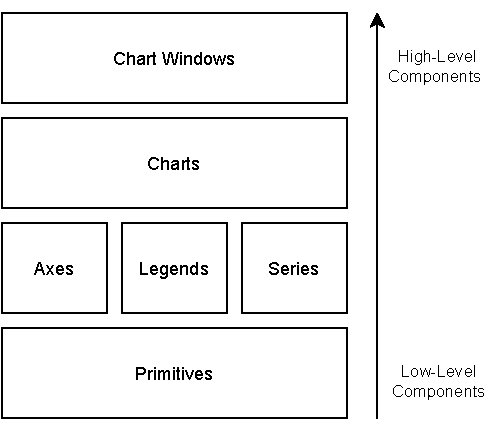
\includegraphics[keepaspectratio,width=\linewidth,height=\fullh / 3]{diagrams/respvis-layers.pdf}
\caption[Component Layers of RespVis]{
  This diagram shows the different layers of components of the RespVis library.
  Layers that are higher in the hierarchy contain increasingly higher-level components that make more assumtions than components in lower layers.
  The lowest level of components are primitives that are merely rendered SVG elements such as \code{<rect>}, \code{<circle>}, and \code{<text>} elements.
  Axes, legends and series are composite components that only contain primitives.
  Charts are composite components that are composed of lower-level primitives or other composite components to form a complete visualization.
  Chart windows are wrapper components around charts, manage their rendering process and provide a toolbar for them.  
  \imgcredit{Image created by the author of this thesis.}
}
\label{fig:Layers}
\end{figure}

\section{Naming Conventions}
\label{sec:NamingConventions}

The naming of entities in RespVis follows the same naming conventions that are used in D3 modules.
In D3-related modules, it is common that entity names start with their general type and are further narrowed down until the exact entity is described accurately.
This convention does not have a name, but it is referred to as "top-down naming" in this work.
An example of the top-down naming convention can be seen in the \code{d3-scale} \parencite{D3Scale} and \code{d3-axis} \parencite{D3Axis} modules, in which entities are called things like \code{scaleLinear}, \code{scaleOrdinal}, \code{axisBottom}, and \code{axisLeft} rather than \code{linearScale}, \code{ordinalScale}, \code{bottomAxis}, and \code{leftAxis}.
Since this is the exact opposite of how these entities would be called in the natural english language, using such names can feel odd for the uninitiated. 
However, the experience of working with APIs following such a naming convention is superior to when they do not.
The reason for this is that users of such APIs can easily discover specialized entities by inputting the general entity type and browsing through code completion suggestions provided by their development tools.
Due to this superiority and to stay consistent with other D3 modules, the decision has been made that entity names in RespVis should also follow this convention.
The public interface of the library is mostly made up of types and functions.
Types are usually written as interfaces and represent the shape of an object. 
Their names are written in \code{PascalCase} and adhere to the top-down naming convention.
They always start with the group a type belongs to and further words are successively added to distinguish gradually more specialized types.
The naming of types can best be demostrated by the different names given to different kinds of bar charts.
Normal bar charts are called \code{ChartBar}, grouped bar charts are called \code{ChartBarGrouped}, and stacked bar charts are called \code{ChartBarStacked}.
The API of RespVis is mainly composed of functions.
Function names are always written in \code{camelCase} and also follow the top-down naming convention.
They always start with the type of object they operate followed by the operation they perform.
Names of functions that create the data of a specific component are always in the form of \code{componentNameData}, such as \code{chartBarData} or \code{chartBarGroupedData}.
The names of functions that render specific components are always in the form of \code{componentNameRender}, such as \code{chartBarRender} or \code{chartBarGroupedRender}. 

% https://github.com/papers-we-love/papers-we-love/blob/master/design/out-of-the-tar-pit.pdf
% https://blog.klipse.tech/databook/2020/10/02/separate-code-data.html


\section{Project Setup}
\label{sec:ProjectSetup}

RespVis is set up as a NodeJS \parencite{NodeJS} project that is hosted as an open-source project on GitHub \parencite{RespVisGitHub}.
The implementation is written in TypeScript and grouped into different modules by thematic affinity. 
These TypeScript source files must be compiled to JavaScript and bundled into one combined package, so that users can import the library in their projects.
To perform this compilation and bundling, the Rollup module bundler \parencite{Rollup} is used.
In addition to the bundled JavaScript library, users are required to import an accompanying CSS file containing default styling for the generated visualizations.
The project also contains examples to demonstrate usage of the library by creating various charts.
These examples are HTML files that import required files and contain JavaScript that invokes RespVis functionality to create and update visualizations.
The build process of the library contains multiple steps involving output directory preparation, bundling of library code and copying of various files to the correct locations in the output directory.
It would be tedious to manually perform all these steps every time the library needs to be rebuilt, and therefore this process is automated using the Gulp \parencite{Gulp} task runner, a task-based workflow automation tool.
The following sections will briefly introduce the setup of RespVis and the tools used in the development process.  

\subsection{Directory Structure}

The goal of this section is to give an overview over the directory structure of the RespVis project.
Roughly summarized, the project contains configuration files for various tools, a \code{src/} directory containing the source code for the whole library and accompanying examples, a \code{node_modules} directory containing the project's cached NodeJS dependencies, and a \code{dist/} directory containing built versions of the library and examples ready for distribution.
The configuration files are only discussed broadly here, as later sections go into more details about the setup of the various tools.
A tree visualization of the whole directory structure, including all important files and directories but excluding individual source files, can be seen in Figure~\ref{fig:RespVisDirTree}.

\begin{figure}[tp]
\centering
\framebox[\textwidth]{%
\begin{minipage}{0.9\textwidth}
  \dirtree{%
  .1 package.json.
  .1 gulpfile.js.
  .1 tsconfig.json.
  .1 src/.
  .2 index.html.
  .2 respvis.css.
  .2 lib/.
  .3 core/.
  .3 legend/.
  .3 bars/.
  .3 points/.
  .3 tooltip/.
  .2 examples/.
  .3 data/.
  .3 vendor/.
  .3 bar.html.
  .3 \dots.
  .1 dist/.
  .2 respvis.js.
  .2 respvis.js.map.
  .2 respvis.min.js.
  .2 respvis.min.js.gz.
  .2 respvis.min.js.map.
  .2 respvis.css.
  .2 index.html.
  .2 examples/.
  .3 data/.
  .3 vendor/.
  .3 bar.html.
  .3 \dots.
  .1 node\_modules.
  }
\end{minipage}
}
\caption[RespVis Directory Structure]{
  The directory structure of RespVis project. 
  Only important files are shown here for readability reasons.
  \imgcredit{Figure created by the author of this thesis.}
}
\label{fig:RespVisDirTree}
\end{figure}

At the root directory of the RespVis project reside the necessary project configuration files for NodeJS, TypeScript and Gulp.
The NodeJS configuration file, \code{package.json}, describes the meta-data of the NodeJS project.
It is used to specify the project's dependencies to other packages and is required for every NodeJS project so that it can be uploaded to the npm package registry \parencite{npm}.
The TypeScript configuration file, \code{tsconfig.json}, specifies the configuration the TypeScript compiler uses to compile the libraries' TypeScript source files into their JavaScript counterparts.
The Gulp configuration file, \code{gulpfile.js}, is used to describe atomic, recurring tasks and compositions of them.
These tasks can then be invoked via the Gulp command line tool to automate otherwise tedious workflow processes.

The \code{src/} directory at the root of the project contains all the implementation files of the library in the \code{src/lib/} directory and examples in the \code{src/examples/} directory.
The \code{src/lib/} directory contains all TypeScript source files of the library.
They have been partitioned into modules formed around thematic affinity of the various components.
The \code{core} module contains the core functionality of the library and is a prerequisite for all the other modules.
It includes the layouter implementation, D3 selection extensions, chart base components, and assorted utility functions that simplify diverse tasks when creating visualizations.
The \code{legend} module contains a basic legend component, which renders a color legend consisting of a title, colored rectangles and corresponding labels.
The \code{tooltip} module contains functions to show and hide tooltips, modify tooltip contents, and position tooltips.
It also contains helper functions for series components that render tooltips, to simplify data creation and rendering of those series, so that tooltip-related code does not have to be repeated in various places.
The \code{bars} and \code{points} modules contain the necessary series, chart and chart window components to render bar, grouped bar, stacked bar and point visualizations. 
At the moment, all these modules are being built into a combined package, but there are plans to distribute them separately to allow users of the library to only import those packages they need to not unnecessarily increase their own bundle sizes with code they do not require.

Beside the \code{src/lib/} directory, the \code{src/} directory also contains the \code{src/examples/} directory, which holds the source files of the developed examples.
These examples are distributed alongside the library files, so they are copied to the \code{dist/examples/} directory upon building the project.
Every example consists of an HTML file that imports all the requirements such as \code{respvis.js} and \code{respvis.css} as well as external dependencies such as D3.
It then invokes the necessary RespVis functionality within a \code{<script>} tag, which is embedded in the body of the document.
In addition to the individual example files, the \code{examples} directory also contains a \code{vendor} directory, which contains third-party dependencies, and a \code{data} directory containing data, which is imported by individual examples to make it reusable.

In addition to configuration files and the \code{src/} directory, the root directory also contains two directories that are automatically generated during the build process.
These are the \code{node_modules/} and \code{dist/} directories.
The \code{node_modules/} directory is a directory that exists in every NodeJS project.
It is created when installing the dependencies of a NodeJS project and contains a cached copy of every direct and indirect dependency.
The \code{dist/} directory is generated by the Gulp build tasks and contains all the files necessary to distribute a built version of the library.

The code of RespVis is distributed as JavaScript bundles of different formats that can be used depending on the situation.
These formats are based on both Immediately Invoked Function Expressions (IIFE) and the more modern ES modules format, both of which are explained in more detail in Section~\ref{sec:Rollup}.
Bundles containing the \code{.js} extension in their file name contain IIFE source code, whereas bundles containing the \code{.mjs} extension contain ES module source code.  
These bundles are also distributed in gradually more minimized versions.
The \code{dist/respvis.[m]js} file contains the unmodified JavaScript bundle that can be used by library consumers who require readable code, \code{dist/respvis.min.[m]js} contains the minified JavaScript bundle, and \code{dist/respvis.min.[m]js.gz} contains the minified JavaScript bundle that has additionally been compressed in the GZIP format \parencite{GZIP}.
Beside these code bundles, the Rollup module bundler has been configured to create source maps for the \code{dist/respvis.[m]js} and \code{dist/respvis.min.[m]js} bundles: \code{dist/respvis.[m]js.map} and \code{dist/respvis.min.[m]js.map}.
These source maps can be interpreted by developer tools in browsers to map from certain instructions in the bundled JavaScript code to the exact instruction in the original TypeScript code.
They are an immense help when developing the library because, without them, debugging in browsers would be virtually impossible.
Since RespVis aims to perform all possible styling in CSS, the distribution also contains a \code{dist/respvis.css} file which contains all the default styles of visualizations created with RespVis. 
Currently, this file is written manually as a whole in the \code{src/} directory and merely copied to the \code{dist/} directory during the build process.
In the future, this process should be improved by employing a CSS preprocessing tool such as SASS \parencite{SASS} so that the CSS can be split into multiple files during development.
Beside the bundled library source code and stylesheets, the \code{dist/} directory also contains usage examples of the library within the \code{dist/examples/} directory.
This directory is identical to the one under \code{src/examples/} because it is merely being copied to the \code{dist/} folder during the build process.

% @misc{GZIP,
%   title={RFC1952: GZIP File Format Specification Version 4.3},
%   author={Deutsch, Peter},
%   year={1996}
% }

% @article{SASS,
%   title={SASS (Syntactically Awesome Style Sheets)},
%   author={O'Donnell, Jane},
%   journal={Journal of Computing Sciences in Colleges},
%   volume={34},
%   number={4},
%   pages={101--102},
%   year={2019},
%   publisher={Consortium for Computing Sciences in Colleges}
% }


\subsection{NodeJS}

NodeJS is a standalone JavaScript runtime built on top of the V8 JavaScript engine \parencite{V8}.
It is an open-source and multi-platform runtime that enables the execution of JavaScript code outside of web browsers.
NodeJS is heavily used for server-side development to unify the technology stack of web developers and allow them to use JavaScript for both client-side and server-side development.
However, with the appropriate project setup, NodeJS can be used for any kind of development.
It can even be set up as a very powerful framework to develop client-side applications, like it has been done in the RespVis library.
One of the most important tools in the NodeJS environment is the npm package manager \parencite{npm}.
It was created in 2009 to simplify the sharing of source code modules and the management of the dependencies of a module.
The npm package registry hosts a huge number of open-source modules for NodeJS projects, which can easily be imported and used to create new ones.

RespVis is developed as a npm package.
Every npm package is configured via a \code{package.json} file.
This file contains all the necessary meta-data of a package to make it identifiable and provide enough information about what the package contains.
It also lists all the dependencies of a package, so they easily be updated and downloaded during the installation process.
A package can include normal dependencies and development dependencies.
The difference between those two types of dependencies is that normal dependencies of a package will always be installed alongside of it, whereas the development dependencies will only be installed when installing a local package.
The \code{package.json} file that is located in the root directory of the RespVis package can be seen in Listing~\ref{list:PackageJSON}.

\begin{samepage}
\lstinputlisting[%
  float=tp,
  aboveskip=\floatsep,
  belowskip=\floatsep,
  xleftmargin=0cm,              % no extra margins for floats
  xrightmargin=0cm,             % no extra margins for floats
  %
  basicstyle=\footnotesize\ttfamily,
  frame=shadowbox,
  numbers=left,
  label=list:PackageJSON,
  caption={[RespVis' \code{package.json} File]%
    The \code{package.json} file of the RespVis library.
    This file contains all the meta-data to describe the package and it's dependencies.
    Keywords and type dependencies have been omitted for readability reasons.
  },
]{listings/package.json}
\end{samepage}

% V8 https://v8.dev/





\subsection{Rollup}
\label{sec:Rollup}

\TODO{Mention tree shaking}

The Rollup module bundler is used to bundle the source code of the RespVis library.
Bundling is used to combine code that is written as multiple smaller modules to make it easier to distribute.
It also takes care of the necessary transformations to bundle code in different formats, without developers having to worry about the details of how their code will be packaged.
All developers have to do is to write their code once in a form that can be parsed by Rollup, and it will perform the necessary actions.

Rollup supports creating bundles in most common module formats like CommonJS, Asynchronous Module Definition (AMD), Universal Module Definition (UMD), Immediately Invoked Function Expressions (IIFE), and ES.
RespVis is distributed as both IIFE and ES modules.
IIFEs have already existed for a long time, as they were used to support modular software designs in JavaScript before more elaborate module formats were defined.
They are anonymous functions that are executed directly after declaring them.
These functions contain the full logic of the module and return an object representing its publicly accessible interface.
This object is usually stored in a variable, to allow interactions with the module after it has been created. 
IIFE modules are plain JavaScript and do not require any modern features to be supported by browser.
They are simply loaded in web documents like any other JavaScript resource via a \code{<script>} element.
The example in Listing~\ref{list:IIFE} was created to demonstrate the IIFE module format. 

ES modules are a more recent addition to JavaScript, as they have only been introduced in ECMAScript 6 \parencite{ECMAScript6}.
They are a native module system that is built on the \code{import} and \code{export} statements, which are widely supported by modern browsers.
Given that the individual modules of the RespVis library are built as ES modules, Rollup mostly only has to merge them to create a valid, combined ES module.
Since ES modules are natively supported by browser they can be loaded directly in a web document using a \code{<script>} element.
However, it is necessary to mark them as modules, so that browsers can interpret them accordingly.
This is done via the \code{type="module"} attribute on the loading \code{<script>} element.


\begin{samepage}
\lstinputlisting[%
  float=tp,
  aboveskip=\floatsep,
  belowskip=\floatsep,
  xleftmargin=0cm,              % no extra margins for floats
  xrightmargin=0cm,             % no extra margins for floats
  %
  basicstyle=\footnotesize\ttfamily,
  frame=shadowbox,
  numbers=left,
  label=list:IIFE,
  caption={[IIFE Module Format]%
    Immediately Invoked Function Expression (IIFE) modules wrap the module code into a function that gets executed immediately after declaring it and returns the public interface of the module.
    Comments were added to show in which files the individual pieces of code reside.
    \code{do-something.js} contains the original code that should be wrapped into an IIFE module, \code{module.js} contains the code of the IIFE module, and \code{application.js} demonstrates the usage of the module.
  },
]{listings/iife.js}
\end{samepage}


The core package of Rollup is only able to create mostly unmodified bundles from JavaScript source files.
Various plugins exist that add frequently-required additional functionality.
There are two kinds of Rollup plugins: bundle plugins, which affect the bundling process, and output plugins, which transform the already bundled code.

The bundle plugins that are used for the bundling of RespVis are the \code{@rollup/plugin-node-resolve}, \code{@rollup/plugin-commonjs}, and \code{@rollup/plugin-typescript} plugins.
The \code{@rollup/plugin-node-resolve} plugin is used to resolve imports from other NodeJS packages that reside in the \code{node_modules} directory.
Since many NodeJS packages are still implemented as CommonJS modules, which are not natively supported by Rollup, the \code{@rollup/plugin-commonjs} plugin has been added to interpret them.
Lastly, the \code{@rollup/plugin-typescript} plugin is used to compile TypeScript source files to JavaScript before bundling them.
The configuration with which the TypeScript compiler is invoked is taken from the \code{tsconfig.json} file at the root directory of the project.

The output plugins used during the bundling process are the \code{rollup-plugin-terser} and \code{rollup-plugin-gzip} plugins.
These plugins do not affect every created bundle.
Instead, they are used to selectively transform the contents of specific bundles.
The \code{rollup-plugin-terser} plugin is used to minify the code of created bundles containing the \code{.min} extension in their file names.
Logically, they are equivalent to non-minified bundles, but they are compressed as much as possible to reduce their file size while still containing valid, although unreadable, JavaScript code. 
Another output plugin used for even stronger minification is the \code{rollup-plugin-gzip} plugin.
This plugin has been applied to all bundles containing the \code{.gz} extension in their file names.
It performs another step of compression on bundles that have already been minified using the \code{rollup-plugin-terser} plugin, by packing them in the GZIP compression format \parencite{GZIP}. 

Another noteworthy thing is that D3 is not included in any of the generated bundles.
The reason for this is that RespVis is designed to be an extension of D3 and, most of the time, an application that wishes to use RespVis will already by relying on it.
If D3 were to be included in the bundle of RespVis, it would unnecessarily be loaded a second time.
This redundancy would cause a needless increase in the bundle size and loading time of the library.
To prevent D3 from being included in the created bundles, all dependencies from D3-related packages are marked as external.

The actual bundling is performed via the JavaScript API of Rollup in the private \code{bundleJS} Gulp task.
This task is executed in various automation processes set up with Gulp, which are explained in more detail in Section~\ref{sec:Gulp}.
The code of the \code{bundleJS} task can be seen in Listing~\ref{list:BundleJS}.
As can be observed in the code, the Rollup API allows the library to be bundled once via the \code{Rollup.rollup} function that returns the created bundle.
This bundle can then be written to the target destination via the \code{Bundle.write} method, which allows the specification of the target bundle format and the plugins used to transform the code before writing it.


\begin{samepage}
\lstinputlisting[%
  float=tp,
  aboveskip=\floatsep,
  belowskip=\floatsep,
  xleftmargin=0cm,              % no extra margins for floats
  xrightmargin=0cm,             % no extra margins for floats
  basicstyle=\footnotesize\ttfamily,
  frame=shadowbox,
  numbers=left,
  label=list:BundleJS,
  caption={[Gulp Task that Bundles the Library Code]%
    The private Gulp task that bundles the code of the RespVis libary.
    Bundling is performed once using the \code{Rollup.rollup} function. 
    After the library has been bundled, it is written multiple times with different configurations using the \code{Bundle.write} method. 
  }
]{listings/bundle-js.js}
\end{samepage}
  


\subsection{Gulp}
\label{sec:Gulp}

\TODO{Add figure of npx gulp --tasks}

Gulp is a task runner that automates workflow processes via a set of named tasks.
It is used to automate processes like building the library and serving the examples on a development server.
Tasks perform a certain operation that needs to be carried out recurringly.
They can perform an atomic operation or represent a composition of other tasks.  
These composite tasks can execute tasks contained in them in a serial or parallel order.
Individual tasks are implemented as JavaScript functions in the Gulp configuration file, \code{gulpfile.js}, which can be found in the root directory of the project.
This approach of favoring code over declarative configuration files means that the person setting up process automation needs to be familiar with JavaScript to do so, in return the possibilities of configuration are endless. 

Tasks in the \code{gulpfile.js} file have been separated into private and public tasks.
Private tasks are simply asynchronous functions that perform a certain action that does not necessarily have to be executed by external entities.
The private Gulp tasks set up in the RespVis project are the \code{bundleJS}, \code{bundleCSS}, \code{copyExamples}, \code{cleanDist}, \code{cleanNodeModules}, and \code{reloadBrowser} tasks.  
Public tasks are also asynchronous functions, but they are exported and are therefore available to be executed via the Gulp command-line interface.
Most public tasks set up in this project are compositions of other tasks or references to them.
The public tasks that are available are the \code{clean}, \code{cleanAll}, \code{build}, and \code{serve} tasks.
The default task that is being executed when no other task is specified via the command-line interface is the \code{serve} task.

Bundling of the library's source code is implemented in the private \code{bundleJS} task. 
It uses the JavaScript API of Rollup to bundle all TypeScript files into IIFE and ES modules of varying levels of minification. 
This task has already been described in detail in Section~\ref{sec:Rollup}, so it wont be discussed further here.
It is executed during the public \code{build} and \code{serve} tasks.

The \code{bundleCSS} task is used to copy the \code{src/respvis.css} file to the \code{dist/} directory.
Since one of the design pillars of RespVis is to style everything possible with CSS, this file contains all the default styles for visualizations created with RespVis.
Currently, this file is written as a whole in the \code{src/} directory and merely copied to the \code{dist/} directory, but there are plans to build this file from different modules using a CSS preprocessor in the future.
Usage of a CSS preprocessor will require an additional bundling step to be performed that compiles individual CSS modules into a merged CSS bundle that can be interpreted by browsers.
This task is executed as part of the public \code{build} and \code{serve} tasks.

The private \code{copyExamples} task copies all the files from the \code{src/examples/} directory to the \code{dist/} directory.
This task is required because the examples are being developed inside the \code{src/} directory and they need to be made available as library distributables.
Another reason for the copying is that the BrowserSync development server is initialized with the \code{dist/} directory as its root and every file that should be viewable on this server must reside somewhere in there.
The \code{copyExamples} task is executed during the public \code{build} and \code{serve} tasks.

The private \code{cleanDist} and \code{cleanNodeModules} tasks are used to respectively delete the \code{dist/} and \code{node_modules/} directories.
The \code{cleanDist} task is exported under a different name as the public \code{clean} task.
This task is necessary because without cleaning the \code{dist/} directory before every rebuild, files from previous builds that might have disappeared in the meantime would cause littering and confusion.
Therefore, this task is being executed as the first step of the \code{build} task.
The public \code{cleanAll} task is composed of the private \code{cleanDist} and \code{cleanNodeModules} tasks.
It is only executed manually when developers choose to delete the currently cached dependencies of the project to reinstall them from scratch.

The public \code{build} task is responsible for building all parts of the project.
It is a composite task that executes the \code{clean}, \code{bundleJS}, \code{bundleCSS}, and \code{copyExamples} tasks.
The \code{clean} task is invoked before all of the other tasks, which are then executed in parallel.
After this task finishes, the \code{dir/} directory will contain all distributable JavaScript and CSS files of the library, as well as the distributable \code{examples/} directory.

To simplify development of RespVis, a Browsersync \parencite{Browsersync} development server is used to host the built distributables.
Browsersync is a useful tool for synchronized browser testing.
It has many features like simulated network throttling, interaction synchronization, and file synchronization that enable simultaneuous testing in multiple environments.
In the setup of RespVis, it is only used for its ability to synchronize and hot-reload files on the fly.
The public \code{serve} task, which is also exported as the default task, initializes a Browsersync development server that serves files from the \code{dist/} directory.
Automatic reloading of the development server is implemented manually via the \code{Gulp.watch} function.
This function enables a task to be executed whenever a change to a file that is matched by the supplied glob pattern is detected.
The \code{serve} task implements three different cases that cause the development server to reload.
Firstly, every time one of the TypeScript files in the \code{src/lib/} directory changes, the \code{bundleJS} task is executed and the browser is reloaded.
Secondly, every time the \code{src/respvis.css} file changes, the \code{bundleCSS} task is executed and the browser is reloaded.
Thirdly, whenever a file in the \code{src/examples/} directory is being changed, the \code{copyExamples} task is executed and the browser is reloaded.

% \TODO{Checkout these resources: bocoup.com/blog/reusability-with-d3, bocoup.com/blog/introducing-d3-chart}

% \TODO{Add software architecture diagram}

% \TODO{Describe relationship to D3}

% \TODO{Describe storing data on elements}

% \TODO{Describe using DOM events for callbacks}

% \TODO{Describe components}



% \section{Components}



% \subsection{Lifecycle}

% events

% updating on data change

% updating on bounds change